\section{Introduction}
Dans le cadre d'un appel à projets lancé par le musée Fabre à Montpellier pour une soirée sous le nom "François-Xavier n’est pas couché", nous avons eu à réaliser un projet qui a pour but de "Révolutionnez le musée" et qui doit être liée à notre domaine d'études.\\
Pour cela, nos enseignants M. Berry et M. Delahaye nous ont proposer de concevoir un dispositif basé sur le nano-ordinateur Raspberry Pi ou sur le microcontrôleur Arduino tout en nous laissant le choix et l'imagination des fonctionnalités et des objectifs de ce dispositif.\\

\begin{wrapfigure}{r}{0.25\textwidth} %cette figure sera affiché à droite
    \centering
    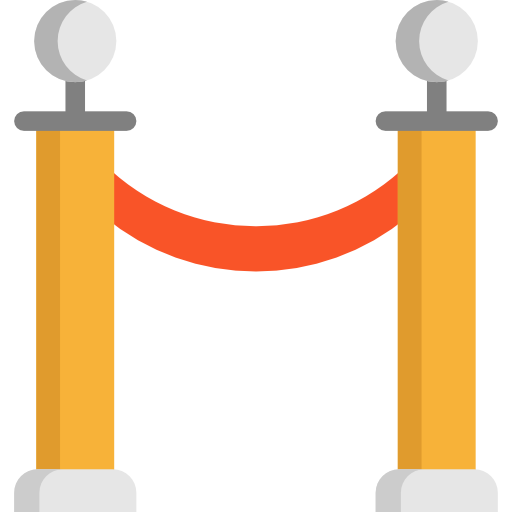
\includegraphics[height=2.5cm]{fencing.png}
\end{wrapfigure}

Dans un musée, la distance minimale entre les oeuvres et les visiteurs est souvent déterminée par une barrière, de sorte que les visiteurs du musée ne peuvent pas la dépasser. Malgrés cela, les oeuvres risquent d’être abîmé par des personnes qui ne respectent pas cette distance.
Pour cela, Nous avons eu l’idée de bien protéger et sécuriser les oeuvres en créant un système de sécurité, capable de détecter les personnes se trouvant dans une zone qui met l’oeuvre en danger, et d’avertir les agents de sécurité du musée. 

\clearpage

